\documentclass[a4paper,14pt]{extarticle}

% Путь до папки с общими шаблонами
\newcommand{\pathToCommonFolder}{/home/denilai/Documents/repos/latex/Common}
% Название работы в титуле
\newcommand{\workname}{Отчет по лабораторной работе №3}
% Название дисциплины в титуле
\newcommand{\discipline}{Проектирование и разработка систем на базе ПЛИС}
% Название кафедры в титуле
\newcommand{\kafedra}{Кафедра Вычислительной техники}
% Тема работы в титуле
\newcommand{\theme}{Проектирование цифрового узла анализатора последовательности и
	его верификация средствами САПР Xilinx ISE 14.х.}
% Должность преподавателя в титуле
\newcommand{\rang}{ассистент}
\newcommand{\signature}{\pathToCommonFolder/denisov-signature}

% ФИО студента в титуле
\newcommand{\studentfio}{К.~Ю.~Денисов}
% ФИО преподавателя в титуле
\newcommand{\teacherfio}{А.~С.~Боронников}


\usepackage{tabularx}


\usepackage{booktabs}
\newcolumntype{b}{X}
\newcolumntype{s}{>{\hsize=.5\hsize}X}
\newcommand{\heading}[1]{\multicolumn{1}{c}{#1}}

% установка размера шрифта для всего документа
%\fontsize{20pt}{18pt}\selectfont
\usepackage{extsizes} % Возможность сделать 14-й шрифт

% Вставка заготовки преамбулы
% Этот шаблон документа разработан в 2014 году
% Данилом Фёдоровых (danil@fedorovykh.ru) 
% для использования в курсе 
% <<Документы и презентации в \LaTeX>>, записанном НИУ ВШЭ
% для Coursera.org: http://coursera.org/course/latex .
% Исходная версия шаблона --- 
% https://www.writelatex.com/coursera/latex/5.3

% В этом документе преамбула

% Для корректного использования русских символов в формулах
% пакеты hyperref и настройки, связанные с ним, стоит загуржать
% перед загрузкой пакета mathtext



% поддержка русских букв
% кодировка шрифта
%\usepackage[T2A]{fontenc} 
\usepackage{pscyr}

% использование ненумеровонного абзаца с добавлением его в содержаниеl

\newcommand{\anonsection}[1]{\section*{#1}\addcontentsline{toc}{section}{#1}}
\newcommand{\sectionunderl}[1]{\section*{\underline{#1}}}


% настройка окружения enumerate
\usepackage{enumitem}
\setlist{noitemsep}
\setlist[enumerate]{labelsep=*, leftmargin=1.5pc}

\usepackage{hyperref}

% сначала ставить \usepackage{extsizes} % Возможность сделать 14-й шрифт
% для корректной установки полей вставлять преамбулу следует в последнюю очередь (но перед дерективой замены \rmdefault)
\usepackage[top=20mm,bottom=25mm,left=35mm,right=20mm]{geometry} % Простой способ задавать поля

\hypersetup{				% Гиперссылки
	unicode=true,           % русские буквы в раздела PDF
	pdftitle={Заголовок},   % Заголовок
	pdfauthor={Автор},      % Автор
	pdfsubject={Тема},      % Тема
	pdfcreator={Создатель}, % Создатель
	pdfproducer={Производитель}, % Производитель
	pdfkeywords={keyword1} {key2} {key3}, % Ключевые слова
	colorlinks=true,       	% false: ссылки в рамках; true: цветные ссылки
	linkcolor=red,          % внутренние ссылки
	citecolor=black,        % на библиографию
	filecolor=magenta,      % на файлы
	urlcolor=blue           % на URL
}

%%% Работа с русским языком
\usepackage{cmap}					% поиск в PDF
\usepackage{mathtext} 				% русские буквы в формулах
\usepackage[T2A]{fontenc}			% кодировка
\usepackage[utf8]{inputenc}			% кодировка исходного текста
\usepackage[english,russian]{babel}	% локализация и переносы
\usepackage{indentfirst}
\frenchspacing

%для изменения названия списка иллюстраций
\usepackage{tocloft}


\renewcommand{\epsilon}{\ensuremath{\varepsilon}}
\renewcommand{\phi}{\ensuremath{\varphi}}
\renewcommand{\kappa}{\ensuremath{\varkappa}}
\renewcommand{\le}{\ensuremath{\leqslant}}
\renewcommand{\leq}{\ensuremath{\leqslant}}
\renewcommand{\ge}{\ensuremath{\geqslant}}
\renewcommand{\geq}{\ensuremath{\geqslant}}
\renewcommand{\emptyset}{\varnothing}

% Изменения параметров списка иллюстраций
\renewcommand{\cftfigfont}{Рисунок } % добавляем везде "Рисунок" перед номером
\addto\captionsrussian{\renewcommand\listfigurename{Список иллюстративного материала}}

\newcommand{\tm}{\texttrademark\ }
\newcommand{\reg}{\textregistered\ }


%%% Дополнительная работа с математикой
\usepackage{amsmath,amsfonts,amssymb,amsthm,mathtools} % AMS
\usepackage{icomma} % "Умная" запятая: $0,2$ --- число, $0, 2$ --- перечисление

%% Номера формул
%\mathtoolsset{showonlyrefs=true} % Показывать номера только у тех формул, на которые есть \eqref{} в тексте.
%\usepackage{leqno} % Нумереация формул слева

%% Свои команды
\DeclareMathOperator{\sgn}{\mathop{sgn}}

%% Перенос знаков в формулах (по Львовскому)
\newcommand*{\hm}[1]{#1\nobreak\discretionary{}
{\hbox{$\mathsurround=0pt #1$}}{}}


% отступ для первого абзаца главы или параграфа
%\usepackage{indentfirst}

%%% Работа с картинками
\usepackage{graphicx}  % Для вставки рисунков
\graphicspath{{images/}{screnshots/}}  % папки с картинками
\DeclareGraphicsExtensions{.pdf,.png,.jpg}
\setlength\fboxsep{3pt} % Отступ рамки \fbox{} от рисунка
\setlength\fboxrule{1pt} % Толщина линий рамки \fbox{}
\usepackage{wrapfig} % Обтекание рисунков текстом

%%% Работа с таблицами
\usepackage{array,tabularx,tabulary,booktabs} % Дополнительная работа с таблицами
\usepackage{longtable}  % Длинные таблицы
\usepackage{multirow} % Слияние строк в таблице

%%% Теоремы
\theoremstyle{plain} % Это стиль по умолчанию, его можно не переопределять.
\newtheorem{theorem}{Теорема}[section]
\newtheorem{proposition}[theorem]{Утверждение}

\theoremstyle{plain} % Это стиль по умолчанию, его можно не переопределять.
\newtheorem{work}{Практическая работа}[part]


 
 
\theoremstyle{definition} % "Определение"
\newtheorem{corollary}{Следствие}[theorem]
\newtheorem{problem}{Задача}[section]
 
\theoremstyle{remark} % "Примечание"
\newtheorem*{nonum}{Решение}



%%% Программирование
\usepackage{etoolbox} % логические операторы

%%% Страница

%	\usepackage{fancyhdr} % Колонтитулы
% 	\pagestyle{fancy}
%   \renewcommand{\headrulewidth}{0pt}  % Толщина линейки, отчеркивающей верхний колонтитул
% 	\lfoot{Нижний левый}
% 	\rfoot{Нижний правый}
% 	\rhead{Верхний правый}
% 	\chead{Верхний в центре}
% 	\lhead{Верхний левый}
%	\cfoot{Нижний в центре} % По умолчанию здесь номер страницы

\usepackage{setspace} % Интерлиньяж
\onehalfspacing % Интерлиньяж 1.5
%\doublespacing % Интерлиньяж 2
%\singlespacing % Интерлиньяж 1

\usepackage{lastpage} % Узнать, сколько всего страниц в документе.

\usepackage{soul} % Модификаторы начертания


\usepackage[usenames,dvipsnames,svgnames,table,rgb]{xcolor}


\usepackage{csquotes} % Еще инструменты для ссылок

%\usepackage[style=authoryear,maxcitenames=2,backend=biber,sorting=nty]{biblatex}

\usepackage{multicol} % Несколько колонок

\usepackage{tikz} % Работа с графикой
\usepackage{pgfplots}
\usepackage{pgfplotstable}

% модуль для вставки рыбы
\usepackage{blindtext}

\usepackage{listings}
\usepackage{color}


% для поворота отдельной страницы. Использовать окружение \landscape
\usepackage{pdflscape} 
\usepackage{rotating} 


\definecolor{mygreen}{rgb}{0,0.6,0}
\definecolor{mygray}{rgb}{0.5,0.5,0.5}
\definecolor{mymauve}{rgb}{0.58,0,0.82}


% пример импорта файла
%\lstinputlisting{/home/denilai/repomy/conf/distributions}

\lstset{
	language=Python,
	basicstyle=\footnotesize,        % the size of the fonts that are used for the code
	numbers=left,                    % where to put the line-numbers; possible values are (none, left, right)
	numbersep=5pt,                   % how far the line-numbers are from the code
	numberstyle=\tiny\color{mygray}, % the style that is used for the line-numbers
	stepnumber=2,                    % the step between two line-numbers. If it's 1, each line will be numbered
	% Tab - 2 пробела
	tabsize=2,    
	% Автоматический перенос строк
	breaklines=true,
	frame=single,
	breakatwhitespace=true,
	title=\lstname 
}



\author{Кирилл Денисов}
\title{Лабораторная работа №2}
\date{\today}

%если не нужна тема работы в отчете, то указать в скобках что-либо, иначе оаставить пустым
\renewcommand{\withouttheme}{}
%если нужна дата представления отчета, то указать в скобках что-либо
%\renewcommand{\withoutsubmissiondate}{1}

% установка полуторного интервала
% \usepackage{setspace}  
% \onehalfspacing

% использовать Times New Roman
\renewcommand{\rmdefault}{ftm}


\begin{document}
	\thispagestyle{empty}
	% Вставка первого титульного листа
	%\newcommand{\withouttheme}{} добавить эту переменную для определения, нужна ли тема
%     {} - нужна
%    {1} - не нужна

%\newcommand{\withoutsubmissiondate}{} добавить эту переменную для определения, нужен ли срок предоставления отчета
%     {} - нужен
%    {1} - не нужен
\begin{center}
	\begin{figure}[h!]
		\begin{center}
		
\includegraphics[width=0.17\linewidth]{\pathToCommonFolder/gerb}
		%\caption{}\label{pic:first}
		%	\vspace{5ex}
		\end{center}	
	\end{figure}
 	\small	МИНОБРНАУКИ РОССИИ \\
	Федеральное государственное бюджетное образовательное учреждение\\
						высшего профессионального образования\\
\normalsize					
\textbf{«МИРЭА – Российский технологический университет»\\
						РТУ МИРЭА}\\
						\noindent\rule{1\linewidth}{1pt}\\
       Институт информационных технологий\\ %\vspace{2ex}
					\kafedra\\
		\vspace{3ex}
			\large \textbf{\workname}  \\
		%\vspace{1ex}
						по дисциплине\\ «\discipline» \\
		\vspace{3ex}
		\if \withouttheme
			\textbf{Тема работы:}\\ <<\theme>>
		\fi
\vspace{3ex}
\small
\begin{table}[h!]
\begin{tabular}{p{0.14\linewidth}p{0.38\linewidth}p{0.25\linewidth}p{0.2\linewidth}}
	\textbf{Выполнил:} & студент группы ИВБО-02-19 & \studentfio &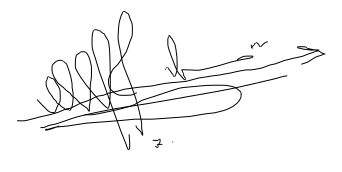
\includegraphics[width=0.8\linewidth]{\signature}\\ \\
	\textbf{Принял:} & \rang & \teacherfio 
\end{tabular}
\end{table}
\end{center}

\begin{flushleft}
	\begin{tabular}{p{0.25\linewidth}l}

		Работа выполена & <<\noindent\rule{2em}{1pt}>>
		                    \noindent\rule{5em}{1pt} 202\noindent\rule{1em}{1pt} \\

		<<Зачтено>> & <<\noindent\rule{2em}{1pt}>>
		\noindent\rule{5em}{1pt} 202\noindent\rule{1em}{1pt} \\

	\end{tabular}
\end{flushleft}

\normalsize
\begin{center}	
\vfill 
Москва 2021
\end{center}

	\newpage
	%\tableofcontents
	\newpage
	%\listoftables
\section*{Постановка задачи}	
%\subsection* {Постановка задачи}

Требуется разработать цифровой узел на основе отладочной платы Digilent Nexys 4,
представляющий собой анализатор фиксированной последовательности логических
сигналов. Узел должен обеспечивать индикацию ожидаемых и вводимых элементов
последовательности посредством входящих в состав отладочной платы семисегментных
индикаторов согласно данному заданию.

Узел должен быть реализован в виде синтезируемой модели на языке Verilog HDL.

Интерфейс верхнего уровня иерархии модели должен состоять из набора сигналов,
представленного на рис. 1.

Автомат должен иметь интерфейс, представленный на рис \ref{fig:fsmexample}.

% TODO: \usepackage{graphicx} required
\begin{figure}[h!]
	\centering
	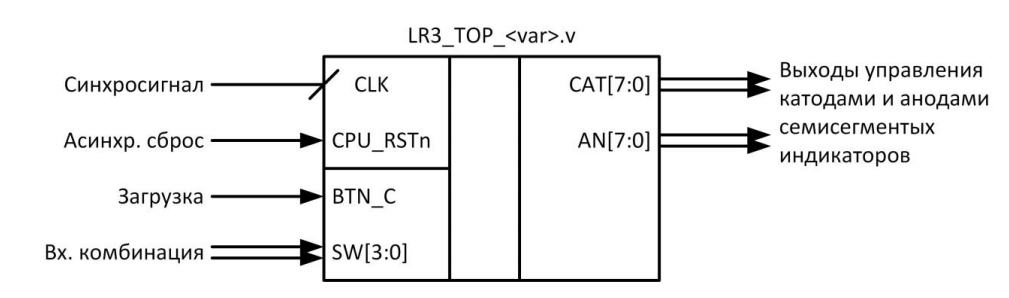
\includegraphics[width=0.7\linewidth]{images/interface-pract3}
	\caption{Интерфейс модели цифрового узла}
	\label{fig:interface-pract3}
\end{figure}


Разрабатываемое устройство является синхронным цифровым узлом,
срабатывающим по восходящим фронтам синхросигнала CLK. Исключение составляет
асинхронный вход сброса CPU\_RSTn, принудительно устанавливающий все регистры
узла в исходное состояние. Подача сигнала сброса на вход узла осуществляется
посредством соответствующей кнопки (CPU\_RSTn) отладочной платы.

Распознавание элементов последовательности осуществляется четверками, т.е.
необходимо обеспечить последовательную загрузку в узел элементов Y c номерами 0-3, 4-
7, 8-B, C-F для успешного распознавания последовательности. При осуществлении ввода
значения, не соответствующего текущему ожидаемому элементу последовательности,
необходимо повторить ввод всей четверки элементов заново




Индикация работы узла посредством двух блоков семисегментных индикаторов для
каждого варианта осуществляется аналогично примеру, представленному на рис. 3 и
подчиняется следующим правилам:
\begin{enumerate}
	\item Левый блок семисегментных индикаторов отображает ожидаемый (младший
	разряд) и введенные (три старших разряда) элементы последовательности в объеме
	распознаваемой четверки.
	\item  Правый блок семисегментных индикаторов отображает предысторию ввода
	комбинаций последовательности. Последняя введенная комбинация отображается в
	младшем разряде блока.
	\item  Не задействованные в текущий момент времени семисегментные индикаторы на
	обоих блоках должны находится в выключенном состоянии.
	\item Обновление отображаемых значений на обоих блоках семисегментных
	индикаторов рекомендуется выполнять с частотой от 60Гц до 200Гц.
\end{enumerate}


\section*{Результат работы}

Реализуем устройство, являющегося синхронным цифровым узлом. Его работу организуем по восходящему фронту синхросигнала, асинхронный сброс --- по нисходящему фронту сигнала CPU\_RSTn. 

\subsection*{Моделирование цифрового устройства}

Приведем таблицу состояний устройства (см. Таблицу \ref{tab:states}). Текущее состояние цифрового устройства зависит от последнего введенного пользователем с помощью движковых переключателей элемента последовательности. 

\begin{table}[htbp]
	\centering
	\caption{Состояния цифрового устройства}
	\begin{tabular}{|c|c|c|c|c|c|c|c|c|c|c|c|c|c|c|c|c|c|}
		\hline
		Состояние & 16& 15&	14	&13	&12&11&	10&	9&	8&	7&	6&	5&	4&	3&	2&	1&	0\\ \hline\hline
		Значение & 0 & 4 & 4 & 8 & 3 & 0 & 7 & 2 & 2 & D & 7 & C & 5 & 2 & A & C&-- \\ \hline\hline
		Разряд & F & E & D & C & B & A & 9 & 8 & 7 & 6 & 5 & 4 & 3 & 2 & 1 & 0 &--\\ \hline
	\end{tabular}

	\label{tab:states}
\end{table}

Приведем граф состояний цифрового устройства (см. Рисунок~\ref{fig:state-graph-pract3}). Переход в следующее состояние происходит только в случае ввода верного элемента последовательности. При неправильном вводе цифровое устройство переходит в ближайшее пройденное состояние, номер которого кратен 4. Номер состояния, в которое перейдет устройство в случае некорректного ввода можно вычислить по формуле 
\[S_{i+1}=(S_i \div 4) \cdot 4\]

% TODO: \usepackage{graphicx} required
\begin{figure}[h!]
	\centering
	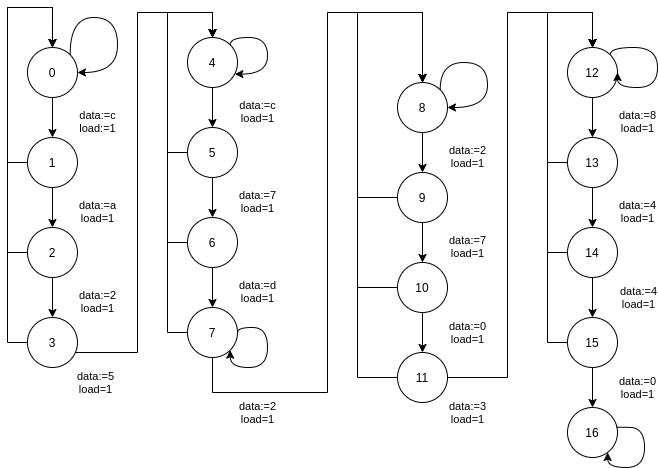
\includegraphics[width=0.7\linewidth]{images/state-graph-pract3}
	\caption{Граф состояний}
	\label{fig:state-graph-pract3}
\end{figure}

%\newpage
Приведем блок схему работы устройства (см. Рисунок~\ref{fig:algorithm-pract3}). Значение Х представляет
собой номер элемента цифровой последовательности, ввод значения которого (Y)
ожидается. Значения Y каждого элемента цифровой последовательности определяются
вариантом задания.

% TODO: \usepackage{graphicx} required
\begin{figure}[h!]
	\centering
	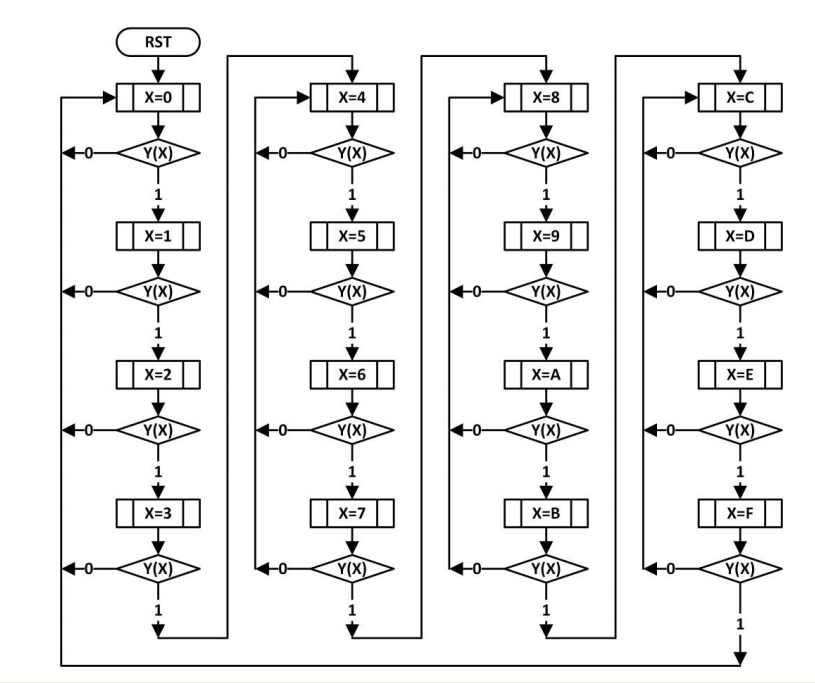
\includegraphics[width=0.68\linewidth]{images/algorithm-pract3}
	\caption{Алгоритм распознавания последовательности}
	\label{fig:algorithm-pract3}
\end{figure}

Приведем структурную схему синхронного цифрового узла (см. Рисунок~\ref{fig:unit-pract3}).

% TODO: \usepackage{graphicx} required
\begin{figure}[h!]
	\centering
	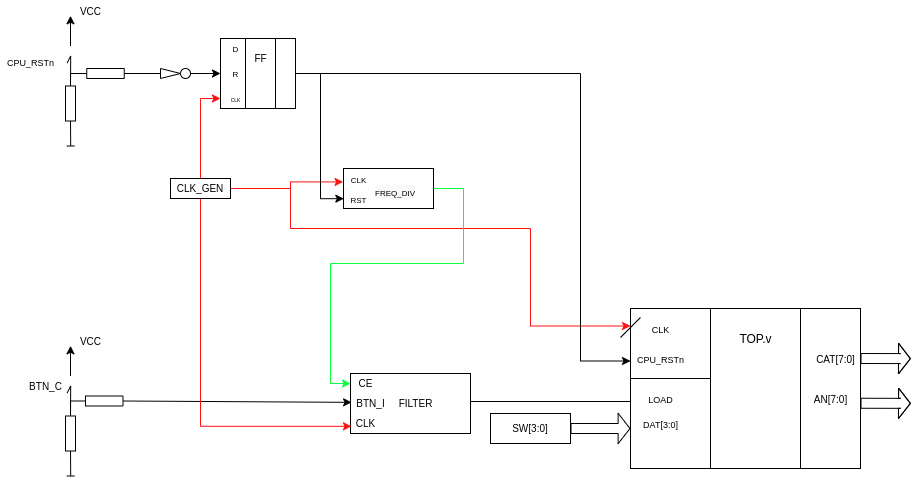
\includegraphics[width=0.8\linewidth]{images/unit-pract3}
	\caption{Структурная схема узла}
	\label{fig:unit-pract3}
\end{figure}


\subsection*{Описание принципа работы}

Опишем главный алгоритм работы цифрового устройства --- контроль ввода шестнадцатеричных чисел с возможностью повторного задания последовательности.

Данный алгоритм описан в файле \texttt{seqAuto.v}. Его содержание приведено в Листинге \ref{lst:seq-auto}.

Сначала производим первоначальную инициализацию переменных, затем, если есть необходимость обновить изображение на дисплее (переменная \texttt{updateDisplay}), начинаем анализировать текущее состояние дисплея и пользовательский ввод. 

Если мы находимся в состоянии, номер которого кратен четырем, то отображаем только левый разряд на левом дисплее. Выводим на это место значение соответствующее значение функции, а в остальные 3 разряда левого дисплея выводим нули.

Если же мы находимся в каком--то другом состоянии, то следует перезаписать все разряды на левом дисплее на один разряд влево, записать в освободившийся разряд записываем очередное значение вектор--функции. 

В конце устанавливаем переменную \texttt{updateDisplay} в нуль. 

Если пользователь подал сигнал на загрузку числа, произведем следующие действия:

Перезапишем все разряды на правом дисплее на один разряд влево, в освободившийся разряд запишем заданное пользователем число. 

Осуществим проверку введенного числа --- сравним его с соответствующим значением вектор--функции. Если пользователь произвел верный ввод, инструментируем переменную состояния автомата (переведем его в следующее состояние). В случае ввода неправильного числа возвращаемся в ближайшее пройденное состояние, номер которого кратен 4. 

В конце устанавливаем переменную \texttt{updateDisplay} в единицу.

\subsection*{Листинг файлов}
Приведем содержание файла seqAuto.v, реализующего главный алгоритм управления цифровым устройством, который был описан в предыдущей секции (см. Листинг \ref{lst:seq-auto}).

\lstinputlisting[caption=Описание главного алгоритма,label=lst:seq-auto]{\pathToScriptsFolder/pract-3/seqAuto.v}

Приведем содержание файла buttonFilter.v, описывающего работу фильтра дребезга, используемого в данной работе для фильтрации цифрового сигнала, приходящего с кнопок ввода (см. Листинг \ref{lst:filter}).


\lstinputlisting[caption=Описание фильтра дребезга,label=lst:filter]{\pathToScriptsFolder/pract-3/buttonFilter.v}

Приведем содержание файла freq\_div.v, описывающего работу делителя частоты, применяемого в данном проекте для снижения выходных характеристик частотного генератора для подбора оптимального режима работы с семисегментными индикаторами (см. Листинг \ref{lst:freq}).

\lstinputlisting[caption=Описание делителя частоты,label=lst:freq]{\pathToScriptsFolder/pract-3/freq_div.v}

Приведем содержание файла NexysDisplay.v, описывающего работу с семисегментыми индикаторами (см. Листинг \ref{lst:n-display}).

\lstinputlisting[caption=Описание модуля работы с семисегментыми индикаторами алгоритма,label=lst:n-display]{\pathToScriptsFolder/pract-3/NexysDisplay.v}

Приведем содержание файла outFunc.v, описывающего представление бинарной вектор--функции, значения которой сравниваются с пользовательским вводом (см. Листинг \ref{lst:func}).

\lstinputlisting[caption=Описание вектор--функции,label=lst:func]{\pathToScriptsFolder/pract-3/outFunc.v}


Приведем содержание файла SevenSegDec.v, описывающего работу сигнального дешифратора для работы с семисегментыми индикаторами  (см. Листинг \ref{lst:decode}).

\lstinputlisting[caption=Описание сигнального дешифратора,label=lst:decode]{\pathToScriptsFolder/pract-3/SevenSegDec.v}


Приведем содержание файла top.v, описывающего работу модуля верхнего уровня, объединяющего все файлы и организующего работу с устройством  (см. Листинг \ref{lst:top}).

\lstinputlisting[caption=Описание модуля верхнего уровня,label=lst:top]{\pathToScriptsFolder/pract-3/top.v}

\subsection*{Эмуляция работы цифрового устройства}

Произведем тестирование работы спроектированного цифрового устройства средствами средствами САПР Xilinx ISE 14. 

% TODO: \usepackage{graphicx} required
\begin{figure}[htpb]
	\centering
	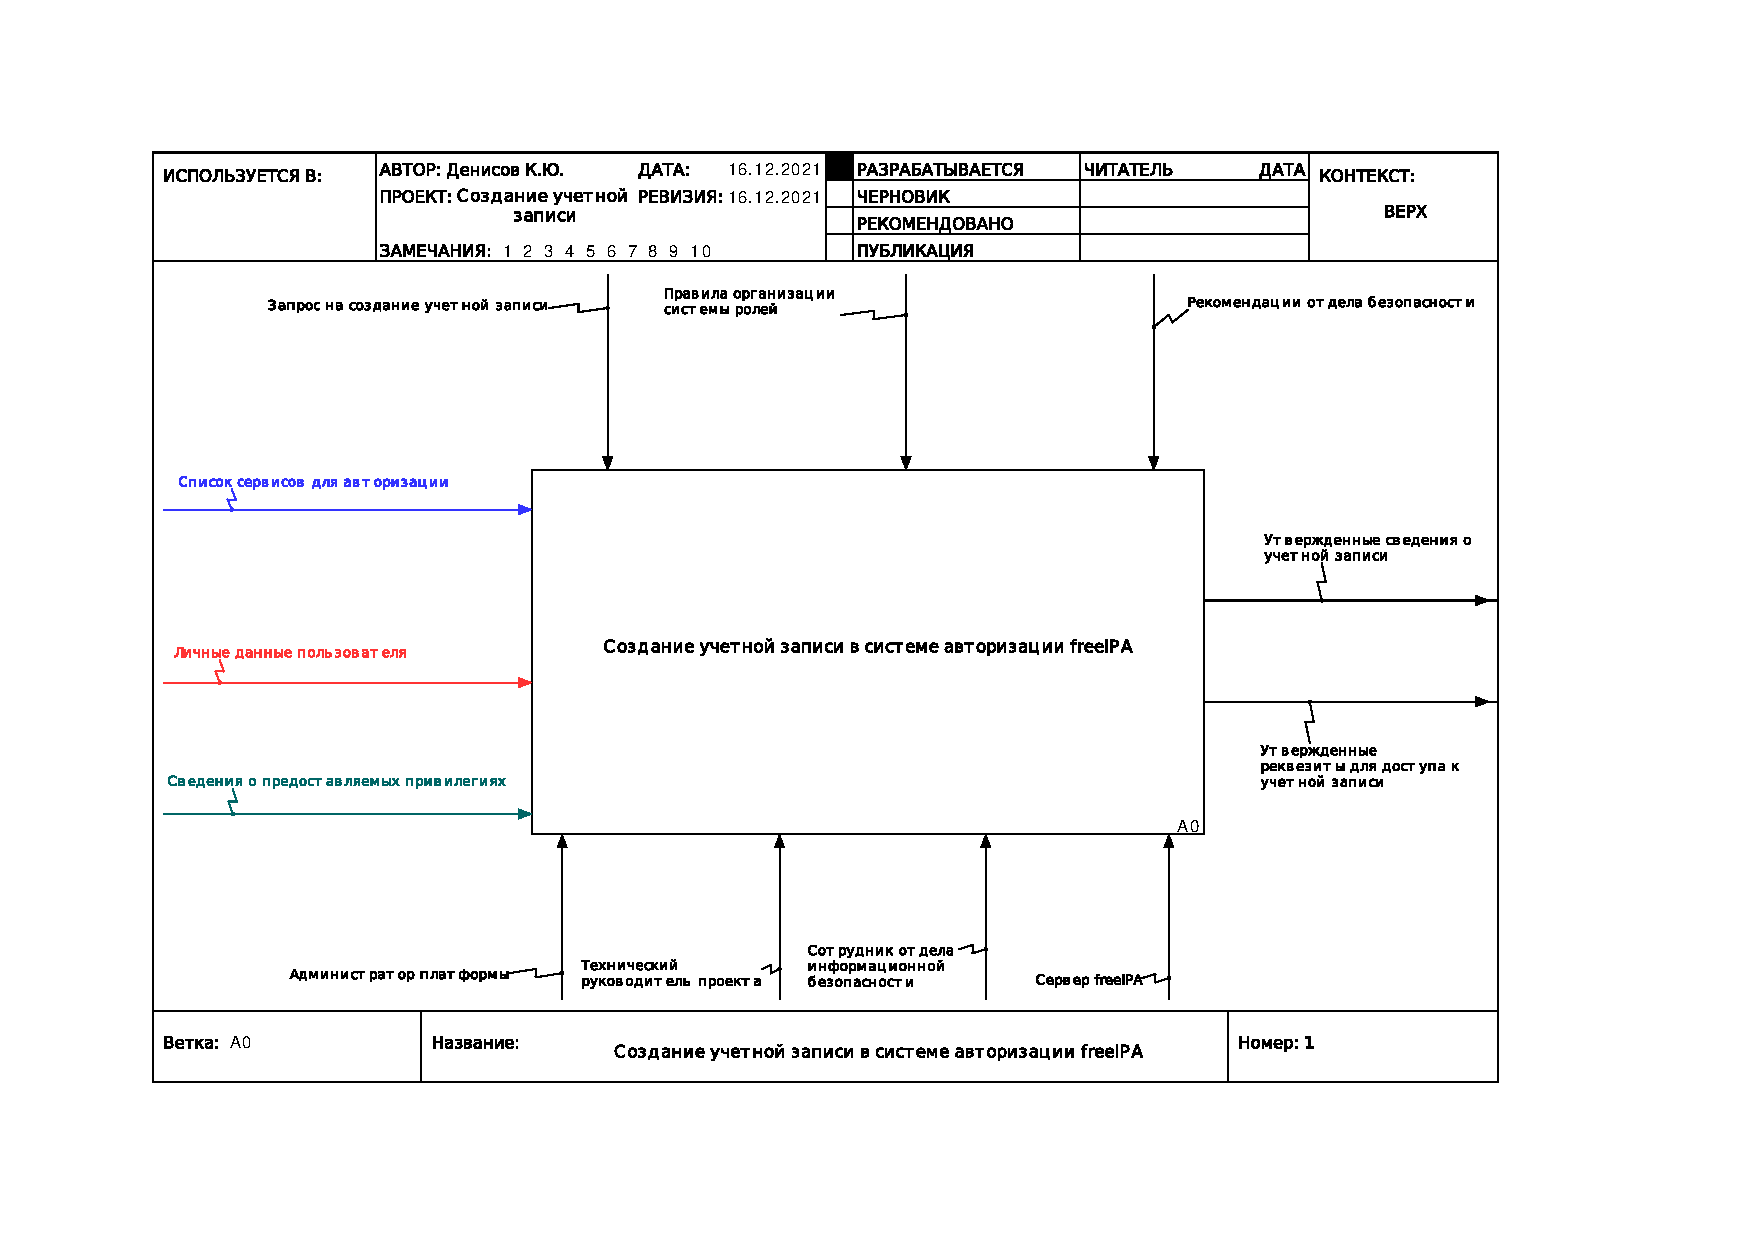
\includegraphics[width=1\linewidth]{images/pract-3/page-1}
	\caption{Эмуляция работы. Часть 1}
	\label{fig:page-1}
\end{figure}
% TODO: \usepackage{graphicx} required
\begin{figure}[htpb]
	\centering
	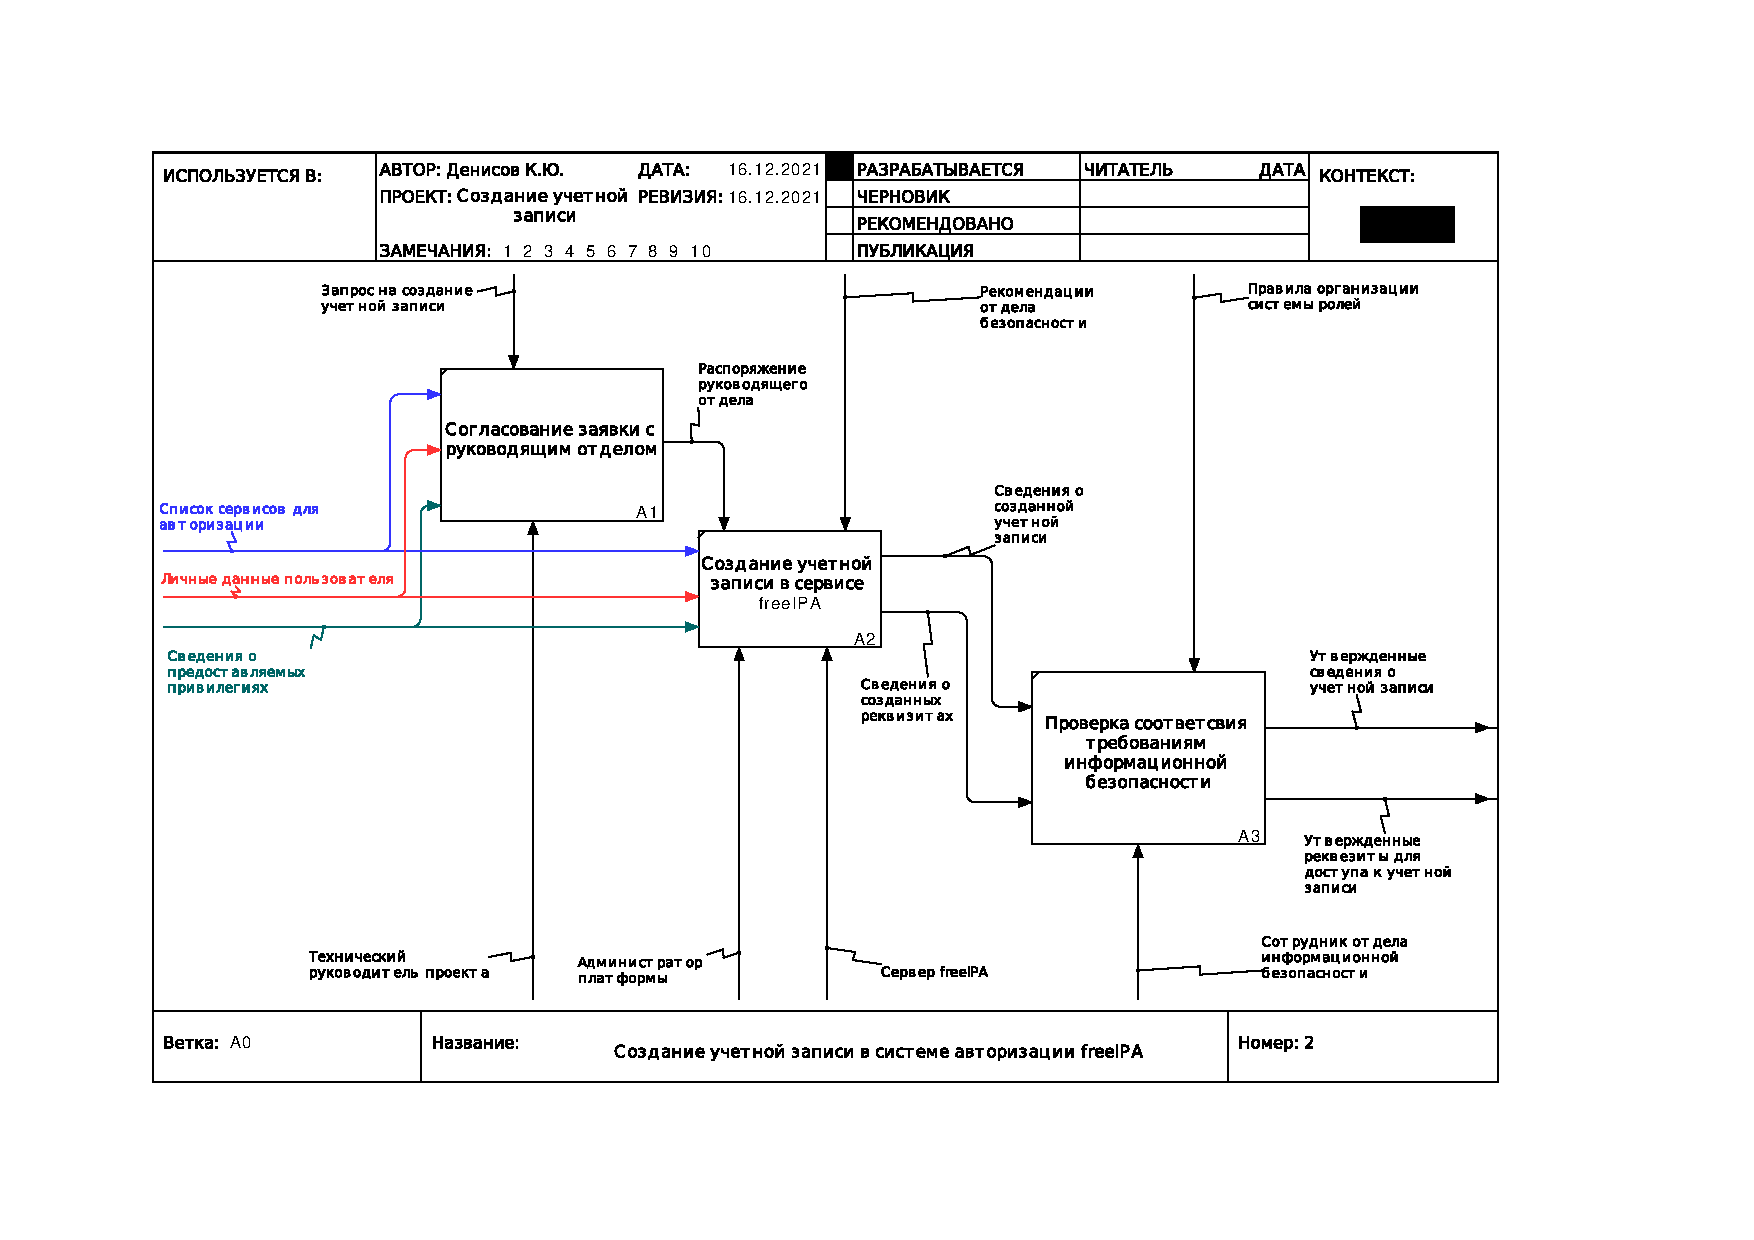
\includegraphics[width=1\linewidth]{images/pract-3/page-2}
	\caption{Эмуляция работы. Часть 2}
	\label{fig:page-2}
\end{figure}
% TODO: \usepackage{graphicx} required
\begin{figure}[htpb]
	\centering
	\includegraphics[width=1\linewidth]{images/pract-3/page-3}
	\caption{Эмуляция работы. Часть 3}
	\label{fig:page-3}
\end{figure}
% TODO: \usepackage{graphicx} required
\begin{figure}[htpb]
	\centering
	\includegraphics[width=1\linewidth]{images/pract-3/page-4}
	\caption{Эмуляция работы. Часть 4}
	\label{fig:page-4}
\end{figure}
% TODO: \usepackage{graphicx} required
\begin{figure}[htpb]
	\centering
	\includegraphics[width=1\linewidth]{images/pract-3/page-5}
	\caption{Эмуляция работы. Часть 5}
	\label{fig:page-5}
\end{figure}
% TODO: \usepackage{graphicx} required
\begin{figure}[htpb]
	\centering
	\includegraphics[width=1\linewidth]{images/pract-3/page-6}
	\caption{Эмуляция работы. Часть 6}
	\label{fig:page-6}
\end{figure}

 
\clearpage
{Вывод: }
В ходе данной практической работы нами были получены общие навыки работы с программным обеспечением Xilinx ISE Design Suite, изучены основы языка Verilog.

С помощью полученных знаний был спроектирован и разработан цифровой узел на основе отладочной платы Digilent Nexys 4, представляющий собой анализатор фиксированной последовательности логических
сигналов. 
\end{document}
